
\subsection{mMAD-based optimization strategies}\label{S:mMAD}

\MAD\ stands for Mean Absolute Deviation. It is a genuine dispersion measure.
It was introduced by Konno and Yamarzaki in 1991 \cite{Konno} as an alternative to more familiar
variance from mean-variance Markovitz model \cite{Markowitz}.
From a numerical point of view, \MAD-based portfolio optimizations can be expressed as LP while
\MV\ (variance) based portfolio optimizations as QP/SOCP problems. Therefore, the perception that an \MAD-based optimization strategy could
be more easily tractable than its \MV\ equivalent.
In its initial form, the \MAD\ dispersion measure was defined as
\begin{equation}
    \MAD(r) = \mE\left[ \left| r - \mE[r]  \right| \right].
\end{equation}
\MAD\ is not a downside dispersion measure per se. Same as variance, it is a central momentum dispersion measure (see Sec.~\ref{CentralM}), penalizing equally the under and over
realizations relative to the mean.

However, once was recognized that
\begin{equation}
    \mE\left[ \left| r - \mE[r] \right| \right] = 2 \mE\left[ \left( \mE[r] - r \right)^+ \right],
\end{equation}
\MAD\ was extended to m-level \MAD\ dispersion measure (for short \mMAD) in 2001 by Michalowski and Ogryczak \cite{Ogryczak}.
\mMAD\ can be defined as the first order \mHMDD, $p=1$ in Eq.~(\ref{hmdd1}), \ie,
\begin{equation}
    \mMAD(r) = \sum_{l=1}^L \cK_l \times \delta^{(1)}_l(r).
    \label{mmad0}
\end{equation}
where $\{\cK_l\}_{l=1,\cdots,L}$ is a positive non-increasing set of coefficients normalized to unit and
$\delta^{(1)}_l$ is the $l$-th level delta-risk of first rank, recursively defined as
\begin{align}
    \delta^{(1)}_1(r) &= \mE \left[ \left( -\br \right)^+ \right], \label{mmad02} \\
    \cdots & \nonumber \\
    \delta^{(1)}_L(r)  &= \mE \left[ \left( -\br - \sum_{j=1}^{L-1} \delta^{(1)}_j \right)^+ \right], \label{mmad01}
\end{align}
with $\br = r - \mE[r]$ the detrended rate of return.

For higher levels, $L>1$, \mMAD\ is a genuine downside dispersion measure, adding more weight to downside observations below the mean.
The weights associated to extreme events are increasing with the size of $L$.

\BackToContents

\subsubsection{mMAD dispersion measure}
The numerical computation of \mMAD, from Eq.~(\ref{mmad0}), is straightforward.
Let $L$ by the highest level involved in the expression of \mMAD. Then,
the set of $\{\delta^{(1)}_l\}_{l=1,\cdots,L}$ is evaluated recursively as
\begin{equation}
    \delta^{(1)}_l = \frac{1}{N}\sum_{i=1}^N \left( -\br_i -\sum_{j=1}^{l-1} \delta^{(1)}_j \right)^+.
    \label{mmad1}
\end{equation}
The $\mMAD$ is given by the sum from Eq.~(\ref{mmad0}).

\BackToContents

\subsubsection{mMAD optimal portfolio}
The optimization is described by Eqs.~(\ref{gg1}) from Sec.~\ref{strategies} point~\ref{OptRisk},
where $\rho$ is given by \mMAD\ from Eq.~(\ref{mmad0}).
It is the following LP problem.

\bigskip
\noindent Minimize over $\{ \{w_k\}_{k=1,\cdots,M}, \{ \eta_l, \{ s_{li} \}_{i=1,\cdots,N} \}_{l=1,\cdots,L} \}$
\begin{subequations}\label{mmad2}
\begin{align}
    &g = \sum_{l=1}^L \cK_l \eta_l, \label{mmad2a} \\
    \st &\frac{1}{N} \sum_{i=1}^N s_{li} = \eta_l, \label{mmad2b} \\
        &s_{li} + \sum_{k=1}^M w_k \br_{ki} + \sum_{j=1}^{l-1} \eta_j \geq 0, \label{mmad2c} \\
        &\sum_{k=1}^M w_k \mu_k \geq \mu, \label{mmad2d} \\
        &\sum_{k=1}^M w_k = 1, \label{mmad2e} \\
        & s_{li} \geq 0, \label{mmad2f} \\
        &\eta_l \geq 0, \label{mmad2h} \\
        & w_k \geq 0, \label{mmad2g}
\end{align}
\end{subequations}

\noindent where $\mu$ from Eq.~(\ref{mmad2d}) is the portfolio targeted expected rate of return, while $\{\mu_k\}_{k = 1,\cdots,M}$
are the portfolio components expected rate of returns.
Then, we have
\begin{subequations}\label{mmad3}
\begin{align}
    \RR &= \sum_{k=1}^M w_k^* \mu_k, \label{mmad3a} \\
    \mMAD &= g^*, \label{mmad3b} \\
    \delta^{(1)}_l &= \eta_l^*, \label{mmad3c}
\end{align}
\end{subequations}

\noindent where $^*$ denotes the solution of LP problem.
In addition to the optimal portfolio weights $\{w_k^*\}_{k=1,\cdots,M}$ and
expected rate of return $\RR$, the
LP solution provides information about the portfolio \mMAD\ and its delta-risk components.

\bigskip
\noindent Here is an example, using the \azapy\ package, of how to compute the \mMAD\ optimal portfolio.
The \mMAD\ time horizon was set to one quarter and the calibration is performed using the prior 3.25 years of
close-adjusted historical prices (default settings).
For more details see the package documentation at \azapydoc.

\lstinputlisting[language=Python]{../PyScripts/MAD_RiskOptim.py}

\BackToContents

\subsubsection{Minimum mMAD portfolio}

Following the result from Sec.~\ref{strategies} point~\ref{MinRisk},
the algorithm to compute the optimal portfolio with minimum \mMAD\ is given by Eqs.~(\ref{mmad2}) where
$\mu$ from r.h.s. of Eq.~(\ref{mmad2d}) is set to a value equal to the smallest expected rate of
return among the portfolio components, \ie\ $\mu=\min_k\{\mu_k\}$.

\bigskip
\noindent Here is an example, using the \azapy\ package, of how to compute the minimum \mMAD\ portfolio.
The \mMAD\ time horizon was set to one quarter and the calibration is performed using the prior 3.25 years of
close-adjusted historical prices (default settings).
For more details see the package documentation at \azapydoc.

\lstinputlisting[language=Python]{../PyScripts/MAD_MinRisk.py}

\BackToContents

\subsubsection{mMAD optimal portfolio for targeted risk value}
This optimization is described by Eqs.~(\ref{gg2}) from Sec.~\ref{strategies} point~\ref{TargetRisk},
where $\rho$ is given by $\mMAD$ from Eq.\ (\ref{mmad0}).
It is the following LP problem.

\bigskip
\noindent Maximize over $\{ \{w_k\}_{k=1,\cdots,M}, \{ \eta_l, \{ s_{li} \}_{i=1,\cdots,N} \}_{l=1,\cdots,L} \}$
\begin{subequations}\label{mmad4}
\begin{align}
    &g = \sum_{k=1}^M \mu_k w_k, \label{mmad4a} \\
    \st &\sum_{l=1}^L\cK_l \eta_l = \mMAD_0, \label{mmad4d} \\
        &\frac{1}{N} \sum_{i=1}^N s_{li} = \eta_l, \label{mmad4b} \\
        &s_{li} + \sum_{k=1}^M w_k \br_{ki} + \sum_{j=1}^{l-1} \eta_j \geq 0, \label{mmad4c} \\
        &\sum_{k=1}^M w_k = 1, \label{mmad4e} \\
        & s_{li} \geq 0, \label{mmad4f} \\
        &\eta_l \geq 0, \label{mmad4h} \\
        & w_k \geq 0, \label{mmad4g}
\end{align}
\end{subequations}

\noindent where $\mMAD_0$ in Eq.~(\ref{mmad4d}) is the portfolio targeted \mMAD\ dispersion value.
Then, we have
\begin{subequations}\label{mmad5}
\begin{align}
    \RR &= g^*, \label{mmad5a} \\
    \delta^{(1)}_l &= \eta_l^*, \label{mmad5b}
\end{align}
\end{subequations}

\noindent where $^*$ denotes the solution of LP problem.
In addition to the optimal portfolio weights $\{w_k^*\}_{k=1,\cdots,M}$ and expected rate of return $\RR$,
the solution of LP problem provides information about the $\mMAD_0$ delta-risk components values,
although, this information is likely to be known at the outset.

\bigskip
\noindent Here is an example, using the \azapy\ package, of how to compute the optimal portfolio
with the same $\mMAD$ as the equal weighted portfolio.
The \mMAD\ time horizon was set to one quarter and the calibration is performed using the prior 3.25 years of
close-adjusted historical prices (default settings).
For more details see the package documentation at \azapydoc.

\lstinputlisting[language=Python]{../PyScripts/MAD_InvNrisk.py}

\BackToContents

\subsubsection{mMAD optimal portfolio for fixed risk-aversion factor}
This optimization is described by Eqs.~(\ref{gg3}) from Sec.~\ref{strategies} point~\ref{RiskAverse},
where $\rho$ is given by \mMAD\ from Eq.~(\ref{mmad0}).
It is the following LP problem.

\bigskip
\noindent Maximize over $\{ \{w_k\}_{k=1,\cdots,M}, \{ \eta_l, \{ s_{li} \}_{i=1,\cdots,N} \}_{l=1,\cdots,L} \}$
\begin{subequations}\label{mmad6}
\begin{align}
    &g = \sum_{k=1}^M w_k\mu_k - \lambda \sum_{l=1}^L \cK_l \eta_l, \label{mmad6a} \\
    \st &\frac{1}{N} \sum_{i=1}^N s_{li} = \eta_l, \label{mmad6b} \\
        &s_{li} + \sum_{k=1}^M w_k \br_{ki} + \sum_{j=1}^{l-1} \eta_j \geq 0, \label{mmad6c} \\
        &\sum_{k=1}^M w_k = 1, \label{mmad6d} \\
        & s_{li} \geq 0, \label{mmad6e} \\
        &\eta_l \geq 0, \label{mmad6g} \\
        & w_k \geq 0, \label{mmad6f}
\end{align}
\end{subequations}

\noindent where $\lambda$ from Eqs.~(\ref{mmad6a}) is the risk-aversion factor.
Then, we have
\begin{subequations}\label{mmad7}
\begin{align}
    \RR &= \sum_{k=1}^M w_k^* \mu_k, \label{mmad7a} \\
    \mMAD &= \frac{\RR - g^*}{\lambda}, \label{mmad7b} \\
    \delta^{(1)}_l &= \eta_l^*, \label{mmad7c}
\end{align}
\end{subequations}

\noindent where $^*$ denotes the solution of LP problem.
In addition to the optimal portfolio weights $\{w_k^*\}_{k=1,\cdots,M}$ and expected rate of return $\RR$,
the LP solution provides information about \mMAD\ and its delta-risk components values.

\bigskip
\noindent Here is an example, using the \azapy\ package, of how to compute the optimal portfolio
for a given value of the risk-aversion factor $\lambda$.
The \mMAD\ time horizon was set to one quarter and the calibration is performed using the prior 3.25 years of
close-adjusted historical prices (default settings).
For more details see the package documentation at \azapydoc.

\lstinputlisting[language=Python]{../PyScripts/MAD_Averse.py}

\BackToContents

\subsubsection{mMAD-Sharpe optimal portfolio - maximization solution}
This optimization targets the maximization of \mMAD-Sharpe ratio. It is based on the
Eqs.~(\ref{gg4}) from Sec.~\ref{strategies} point~\ref{MaxSharpe}, where $\rho$ is given by \mMAD\ from Eq.~(\ref{mmad0}).
The optimization can be formulated as an LP problem if Eq.~(\ref{gg4b}) can be linearized.
In our case the linearization is straightforward. Introducing the following
variable transformations $\bw_k = t w_k$, $\bs_{li} = t s_{li}$ and $\bbeta_l = t \eta_l$, the LP
problem can be written as follows.

\bigskip
\noindent Maximize over $\{ \{\bw_k\}_{k=1,\cdots,M}, \{ \bbeta_l, \{ \bs_{li} \}_{i=1,\cdots,N} \}_{l=1,\cdots,L}, t \}$
\begin{subequations}\label{mmad8}
\begin{align}
    &g =\sum_{k=1}^M \mu_k \bw_k - \mu_0 t, \label{mmad8a} \\
    \st &\sum_{l=1}^L \cK_l \bbeta_l = 1, \label{mmad8d} \\
        &\frac{1}{N} \sum_{i=1}^N \bs_{li} = \bbeta_l, \label{mmad8b} \\
        &\bs_{li} + \sum_{k=1}^M \bw_k \br_{ki} + \sum_{j=1}^{l-1} \bbeta_j \geq 0, \label{mmad8c} \\
        &\sum_{k=1}^M \bw_k - t = 0, \label{mmad8e} \\
        &t \geq 0, \label{mmad8i} \\
        &\bs_{li} \geq 0, \label{mmad8f} \\
        &\bbeta_l \geq 0, \label{mmad8h} \\
        &\bw_k \geq 0, \label{mmad8g}
\end{align}
\end{subequations}

\noindent where $\mu_0$ from Eq.~(\ref{mmad8a}) is the risk-free rate accessible to the investor.
Then, we have
\begin{subequations}\label{mmad9}
\begin{align}
    w_k &= \frac{\bw_k^*}{t^*} , \label{mmad9a} \\
    \RR &= \frac{g^*}{t^*} + \mu_0, \label{mmad9b} \\
    \Sharpe &= g^*, \label{mmad9c} \\
    \mMAD &= \frac{1}{t^*}, \label{mmad9d} \\
    \delta^{(1)}_l &= \frac{\bbeta_l^*}{t^*}, \label{mmad9e}
\end{align}
\end{subequations}

\noindent where $^*$ denotes the solution of LP problem.
In addition to the optimal portfolio weights $\{w_k\}_{k=1,\cdots,M}$, expected rate of return $\RR$ and
\mMAD-Sharpe ratio $\Sharpe$,
the LP solution provides information about \mMAD\ and its delta-risk components.

\bigskip
\noindent Here is an example, using the \azapy\ package, of how to compute the \mMAD-Sharpe optimal portfolio using the maximization
of \mMAD-Sharpe ratio.
The \mMAD\ time horizon was set to one quarter and the calibration is performed using the prior 3.25 years of
close-adjusted historical prices (default settings).
For more details see the package documentation at \azapydoc.

\lstinputlisting[language=Python]{../PyScripts/MAD_Sharpe.py}

\BackToContents


\subsubsection{mMAD-Sharpe optimal portfolio - minimization solution}
This optimization targets the minimization of the inverse of \mMAD-Sharpe ratio.
It is described by Eqs.~(\ref{gg8}) from Sec.~\ref{strategies} point~\ref{MinSharpe}, where
$\rho$ is given by \mMAD\ from Eq.~(\ref{mmad0}).
The optimization can be formulated as an LP problem if Eq.~(\ref{gg8a}) can be linearized. This can be achieved by
introducing the variable transformations
$\bw_k = t w_k$, $\bs_{li} = t s_{li}$ and $\bbeta_l = t \eta_l$.
Then, the LP problem can be written as follows.

\bigskip
\noindent Minimize over $\{ \{\bw_k\}_{k=1,\cdots,M}, \{ \bbeta_l, \{ \bs_{li} \}_{i=1,\cdots,N} \}_{l=1,\cdots,L}, t \}$
\begin{subequations}\label{mmad10}
\begin{align}
    &g = \sum_{l=1}^L \cK_l \bbeta_l, \label{mmad10a} \\
    \st &\frac{1}{N} \sum_{i=1}^N \bs_{li} = \bbeta_l, \label{mmad10b} \\
        &\bs_{li} + \sum_{k=1}^M \bw_k \br_{ki} + \sum_{j=1}^{l-1} \bbeta_j \geq 0, \label{mmad10c} \\
        &\sum_{k=1}^M \mu_k \bw_k -\mu_0 t = 1, \label{mmad10d} \\
        &\sum_{k=1}^M \bw_k - t = 0, \label{mmad10e} \\
        & t \geq 0, \label{mmad10h} \\
        &\bs_{li} \geq 0, \label{mmad10f} \\
        &\bbeta_l \geq 0, \label{mmad10i} \\
        &\bw_k \geq 0, \label{mmad10g}
\end{align}
\end{subequations}

\noindent where $\mu_0$ from Eq.~(\ref{mmad10d}) is the risk-free rate accessible to the investor.
Then, we have
\begin{subequations}\label{mmad11}
\begin{align}
    w_k &= \frac{\bw_k^*}{t^*} , \label{mmad11a} \\
    \RR &= \frac{1}{t^*} + \mu_0, \label{mmad11b} \\
    \Sharpe &= \frac{1}{g^*}, \label{mmad11c} \\
    \mMAD &= \frac{g^*}{t^*}, \label{mmad11d} \\
    \delta^{(1)}_l &= \frac{\bbeta_l^*}{t^*} , \label{mmad11e}
\end{align}
\end{subequations}

\noindent where $^*$ denotes the solution of LP problem.
In addition to the optimal portfolio weights $\{w_k\}_{k=1,\cdots,M}$, expected rate of return $\RR$ and
\mMAD-Sharpe ratio $\Sharpe$,
the LP solution provides information about \mMAD\ and its delta-risk components.


\bigskip
\noindent Here is an example, using the \azapy\ package, of how to compute the \mMAD-Sharpe optimal portfolio using the minimization
of the inverse of \mMAD-Sharpe ratio.
The \mMAD\ time horizon was set to one quarter and the calibration is performed using the prior 3.25 years of
close-adjusted historical prices (default settings).
For more details see the package documentation at \azapydoc.

\lstinputlisting[language=Python]{../PyScripts/MAD_InvSharpe.py}

\BackToContents

\subsubsection{mMAD frontiers}

Here is an example of how to compute the \mMAD\ frontiers using the \azapy\
package. The \mMAD\ time horizon was set to one quarter and the calibration is performed using the prior 3.25 years of
close-adjusted historical prices (default settings).
For more details see the package documentation at \azapydoc.

The script will produce the plots in Figs. \ref{MAD_fig1a} and \ref{MAD_fig1b}
for historical data collected up to 2021-07-27.


\lstinputlisting[language=Python]{../PyScripts/MAD_frontiers.py}

\begin{figure}[H]
\centering
\begin{subfigure}{.5\textwidth}
  \centering
  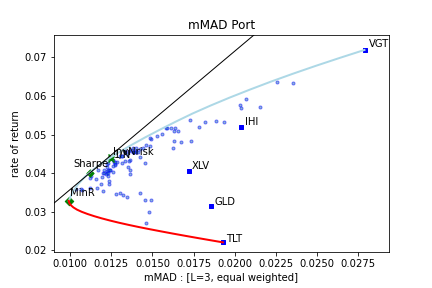
\includegraphics[width=.95\linewidth]{../figs/mMADFrontier1.png}
  \caption{Rate of return vs. \mMAD}
  \label{MAD_fig1a}
\end{subfigure}%
\begin{subfigure}{.5\textwidth}
  \centering
  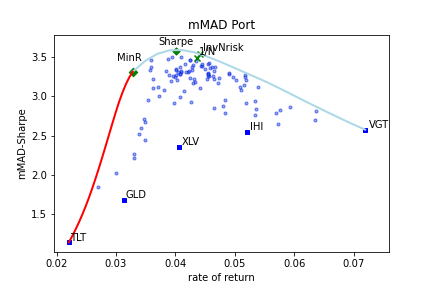
\includegraphics[width=.95\linewidth]{../figs/mMADFrontier2.png}
  \caption{\mMAD-Sharpe vs. rate of return}
  \label{MAD_fig1b}
\end{subfigure}
\caption{\mMAD : [L=3, equal weighted]  frontiers.}
\label{MAD_fig1}
\end{figure}

\BackToContents

\subsubsection{Backtesting mMAD-Sharpe optimal portfolio}

Here is an example, using \azapy\ package, of computing a portfolio backtesting.
For this example, we have chosen a portfolio quarterly rebalanced according
to the maximization of \mMAD-Sharpe ratio. At each rebalancing date,
the portfolio weights
are calibrated based on 3.25 years of prior historical market data.

Other rebalancing strategies can be considered
by changing the value of {\it rtype} parameter in the call of {\it set\_model} function below.
For more details see the package documentation at \azapydoc.

\lstinputlisting[language=Python]{../PyScripts/MAD_Port.py}

\begin{figure}[H]
    \centering
    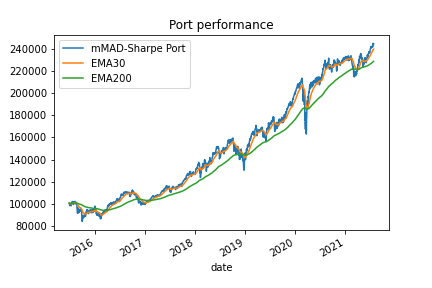
\includegraphics[width=.95\linewidth]{../figs/Port_mMAD_Sharpe.png}
    \caption{Backtesting of quarterly rebalanced \mMAD-Sharpe optimal portfolio,
    \mMAD\ : [L=3, equal weighted].}
    \label{MAD_Port_fig}
\end{figure}

\BackToContents



